%%%%%%%%%%%%%%%%%%%%%%%%%%%%%%%%%%%%%%%%%
% Beamer Presentation
% LaTeX Template
% Version 1.0 (10/11/12)
%
% This template has been downloaded from:
% http://www.LaTeXTemplates.com
%
% License:
% CC BY-NC-SA 3.0 (http://creativecommons.org/licenses/by-nc-sa/3.0/)
%
%%%%%%%%%%%%%%%%%%%%%%%%%%%%%%%%%%%%%%%%%

%----------------------------------------------------------------------------------------
%	PACKAGES AND THEMES
%----------------------------------------------------------------------------------------

\documentclass[t]{beamer}

\mode<presentation> {

% The Beamer class comes with a number of default slide themes
% which change the colors and layouts of slides. Below this is a list
% of all the themes, uncomment each in turn to see what they look like.

%\usetheme{default}
%\usetheme{AnnArbor}
%\usetheme{Antibes}
%\usetheme{Bergen}
%\usetheme{Berkeley}
%\usetheme{Berlin}
%\usetheme{Boadilla}
%\usetheme{CambridgeUS}
%\usetheme{Copenhagen}
%\usetheme{Darmstadt}
%\usetheme{Dresden}
%\usetheme{Frankfurt}
%\usetheme{Goettingen}
%\usetheme{Hannover}
%\usetheme{Ilmenau}
%\usetheme{JuanLesPins}
%\usetheme{Luebeck}
\usetheme{Madrid}
%\usetheme{Malmoe}
%\usetheme{Marburg}
%\usetheme{Montpellier}
%\usetheme{PaloAlto}
%\usetheme{Pittsburgh}
%\usetheme{Rochester}
%\usetheme{Singapore}
%\usetheme{Szeged}
%\usetheme{Warsaw}

% As well as themes, the Beamer class has a number of color themes
% for any slide theme. Uncomment each of these in turn to see how it
% changes the colors of your current slide theme.

%\usecolortheme{albatross}
%\usecolortheme{beaver}
%\usecolortheme{beetle}
%\usecolortheme{crane}
%\usecolortheme{dolphin}
%\usecolortheme{dove}
%\usecolortheme{fly}
%\usecolortheme{lily}
%\usecolortheme{orchid}
%\usecolortheme{rose}
%\usecolortheme{seagull}
%\usecolortheme{seahorse}
%\usecolortheme{whale}
%\usecolortheme{wolverine}

%\setbeamertemplate{footline} % To remove the footer line in all slides uncomment this line
%\setbeamertemplate{footline}[page number] % To replace the footer line in all slides with a simple slide count uncomment this line

%\setbeamertemplate{navigation symbols}{} % To remove the navigation symbols from the bottom of all slides uncomment this line
}

\usepackage{graphicx} % Allows including images
\usepackage{booktabs} % Allows the use of \toprule, \midrule and \bottomrule in tables

%----------------------------------------------------------------------------------------
%	TITLE PAGE
%----------------------------------------------------------------------------------------

\title[uC101]{uC101: Introduction to Microcontrollers / Interfacing with the real world} % The short title appears at the bottom of every slide, the full title is only on the title page

\author{Josh Johnson} % Your name
\institute[] % Your institution as it will appear on the bottom of every slide, may be shorthand to save space
{ \\ % Your institution for the title page
\medskip
\textit{} % Your email address
}
\date{13/5/2019} % Date, can be changed to a custom date

\begin{document}

\begin{frame}
\titlepage % Print the title page as the first slide
\end{frame}

%----------------------------------------------------------------------------------------
%	PRESENTATION SLIDES
%----------------------------------------------------------------------------------------

\section{Subsection Example} % A subsection can be created just before a set of slides with a common theme to further break down your presentation into chunks

\begin{frame}
\frametitle{Overview}
\begin{itemize}
\item Assembly of Hardware
\item Microcontroller 101
\item Tools
\item Bit shifting, logical operations
\item Demos
\begin{itemize}
	\item Blink
	\item Button
	\item RGB LED (PWM)
	\item Rotary Encoder
	\item UART
	\item Charlieplexing
\end{itemize}
	

\end{itemize}
\vspace{20mm}
Project Files: \url{github.com/joshajohnson/CBRhardware}\\
\end{frame}

%----------------------------------------------------------------------------------------

\begin{frame}[t]
\frametitle{Assembly of Hardware}

\begin{figure}
	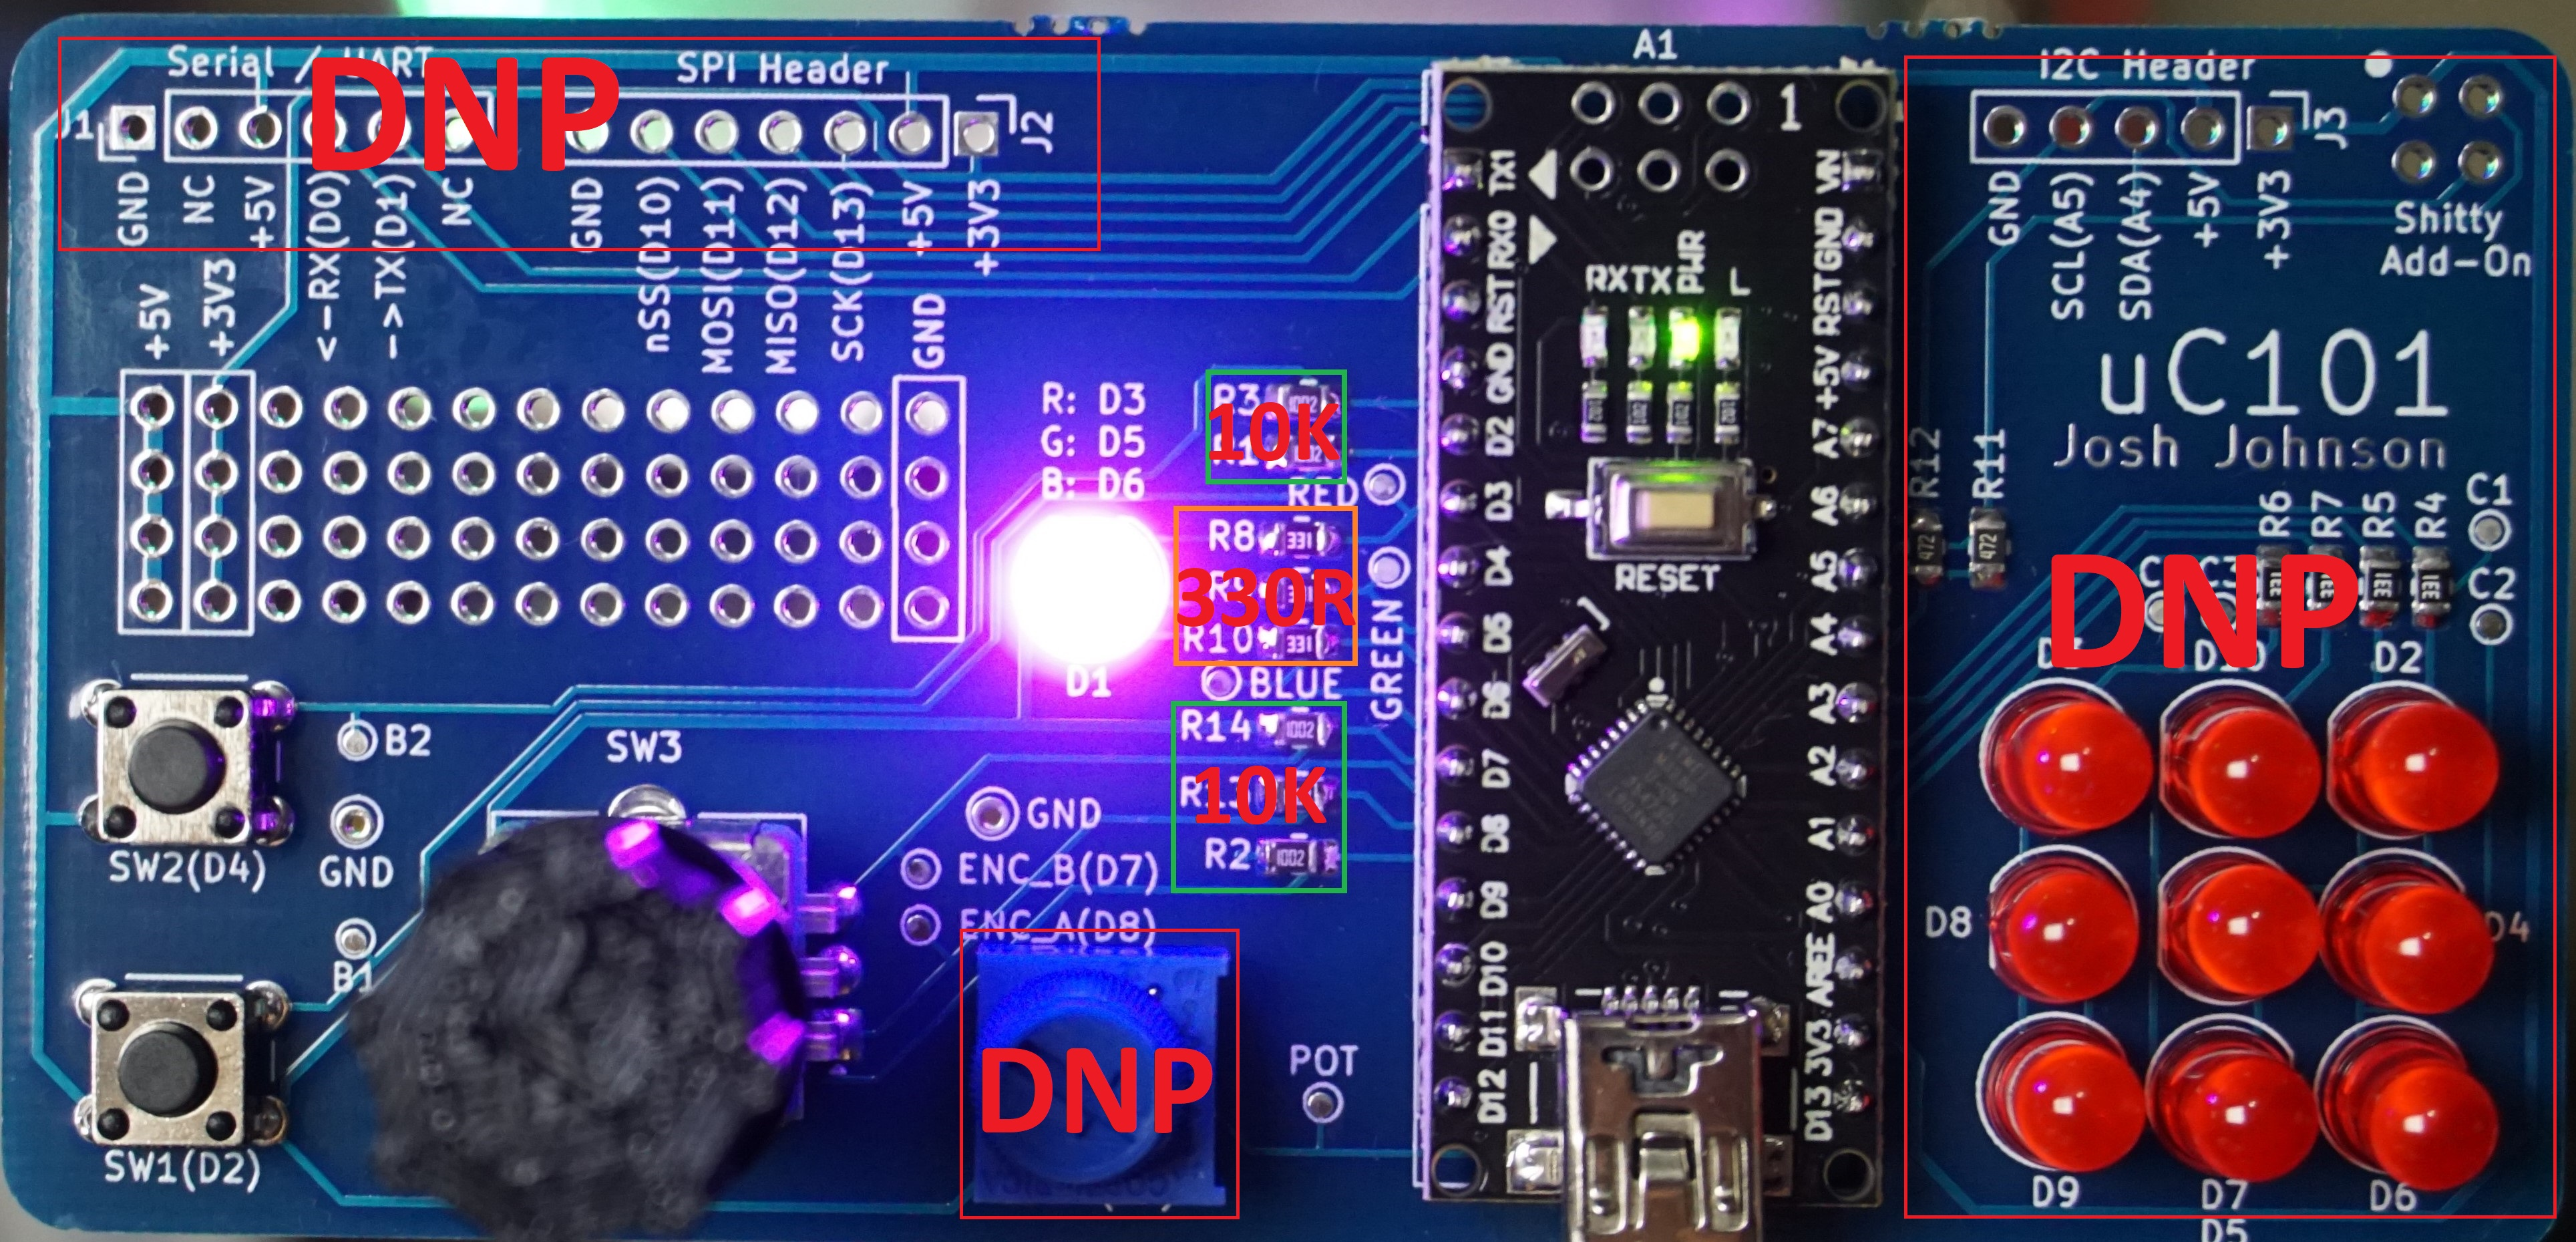
\includegraphics[width=1\linewidth]{hardware.jpg}
\end{figure}

\end{frame}

%----------------------------------------------------------------------------------------

\begin{frame}[t]
\frametitle{Microcontroller 101}

\textbf{What is a microcontroller?} 

\begin{figure}
	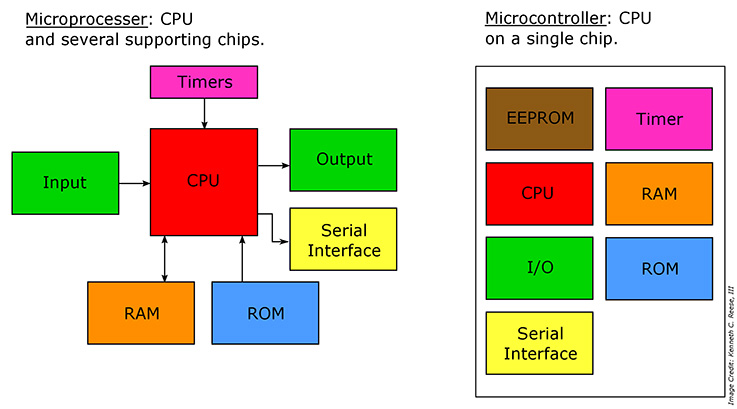
\includegraphics[scale=0.4]{microProcessorVsController.jpg}
\end{figure}

\end{frame}

%----------------------------------------------------------------------------------------

\begin{frame}[t]
\frametitle{Microcontroller 101}

\textbf{Common Options} 

\begin{columns}
	\column{.2\textwidth}
	8 bit
	\begin{itemize}
		\item ATtiny
		\item ATmega \\(Atmel / \\Microchip)
		\item PIC \\(Microchip)
	\end{itemize}

	\column{.2\textwidth}
	16 bit
	\begin{itemize}
		\item MSP430 (TI)
	\end{itemize}
	
	
	\column{.3\textwidth}
	32 bit
	\begin{itemize}
		\item STM32 (ST)
		\item SAM (Atmel/Microchip)
		\item nRF5x (Nordic Semi)
		\item ESP8266/32 (Espressif)
		\item CCxxxx (TI)
		\item LPCxxxx (NXP)
		\item PIC32 (Microchip)
	\end{itemize}

	\column{.29\textwidth}
	32 bit ARM cores
	\begin{itemize}
		\item Cortex-M0/M0+
		\item Cortex-M1 (FPGA only)
		\item Cortex-M3
		\item Cortex-M4 (M3 + DSP + FPU)
		\item ...
		
	\end{itemize}
	
\end{columns}

\end{frame}

%----------------------------------------------------------------------------------------


\begin{frame}[t]
\frametitle{Microcontroller 101}

\textbf{How to choose?}
\begin{itemize}
	\item Compute power
	\begin{itemize}
		\item 8 bit vs 32 bit
		\item DSP / FPU
	\end{itemize} 
	\item Peripherals 
	\begin{itemize}
		\item Wireless
			\begin{itemize}
			\item WiFi
			\item Bluetooth
			\item LoRa
			\item Cellular
		\end{itemize} 
		\item USB
		\item ADC
		\item Ethernet
		\item CAN
		\item Number of SPI/UART/I2C/Timers
	\end{itemize} 
	
\end{itemize} 



\end{frame}

%----------------------------------------------------------------------------------------

\begin{frame}[t]
\frametitle{Microcontroller 101}
\textbf{ATmega328p Architecture} 
\begin{figure}
	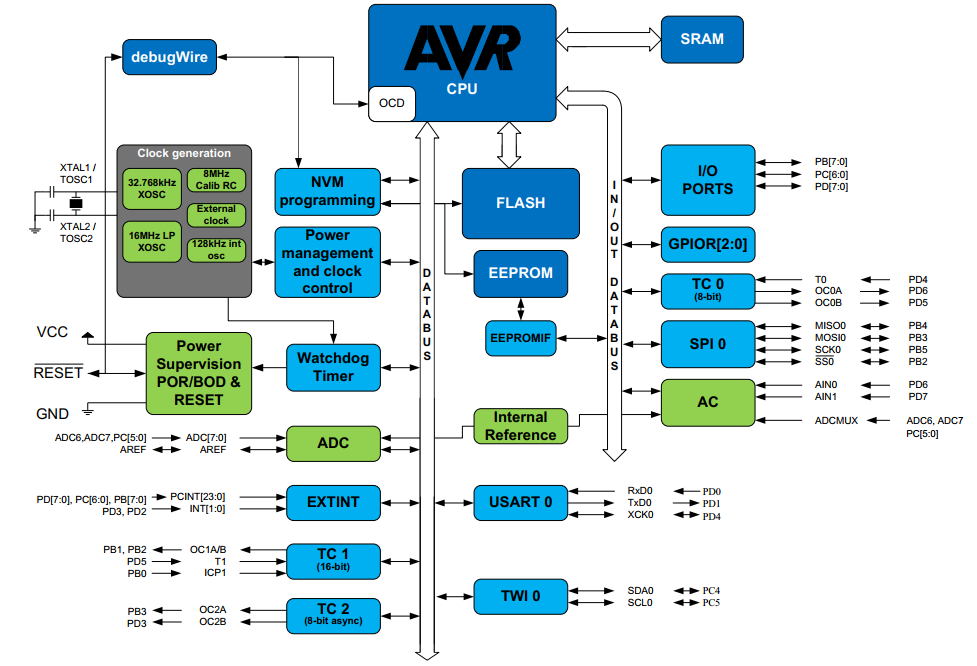
\includegraphics[scale=0.4]{328pArchitecture.png}
\end{figure}

\end{frame}


%----------------------------------------------------------------------------------------

\begin{frame}
\frametitle{The End}
Links to resources: \texttt{uC101/README.md}
\vspace{5mm}

\textbf{Next Month}
\begin{itemize}
	\item Breadboard to Printed Circuit Board
	\item Mechanical Design Considerations	
\end{itemize}

\vspace{20mm}
Say Hello! \\
BSidesCbr Slack: josh\\
Twitter: @\textunderscore joshajohnson\\
Email: josh@joshajohnson.com\\
\vspace{4mm}

Project Files: \url{github.com/joshajohnson/CBRhardware}\\\end{frame}


\end{document} 